%==============================================================================
% PAPER 3, CHAPTER 3: Emergent Geometry from Field Dynamics
% Target: ~320 lines with 60-75 marginal notes and 5 TikZ diagrams
%==============================================================================

\chapter{Emergent Geometry from Field Dynamics}
\label{ch:p3:emergent_geometry}

%------------------------------------------------------------------------------
% OPENING NARRATIVE: Wheeler's Geometrodynamics
%------------------------------------------------------------------------------

\section*{Geometry Tells Matter How to Move}

In the 1960s, physicist John Archibald Wheeler coined the term "geometrodynamics" to capture a radical vision: spacetime geometry is not a fixed stage but an active participant in physics, shaped by and shaping the matter and energy it contains.
\marginhistory{Wheeler's 1960s geometrodynamics program sought to derive all of physics from geometry alone. His aphorism: "Spacetime tells matter how to move; matter tells spacetime how to curve."}

Wheeler's vision goes further: what if geometry itself \textit{emerges} from more fundamental dynamics? Rather than assuming spacetime exists as given, perhaps it crystallizes from underlying quantum fields like ice from water---a phase transition producing the smooth geometry we observe.
\marginphysics{Emergent spacetime: geometry as collective phenomenon arising from microscopic degrees of freedom, analogous to thermodynamics emerging from statistical mechanics.}

This chapter explores mechanisms by which geometric structures emerge from field configurations: how metrics arise from field gradients, how dimensions become effective through renormalization, and how the holographic principle suggests spacetime itself may be a projection of boundary dynamics.

%------------------------------------------------------------------------------
\section{Metric Tensor Emergence from Field Configurations}
\label{sec:p3:metric_emergence}
%------------------------------------------------------------------------------

\subsection{Field Gradients Generating Metrics}

Consider a scalar field $\phi(\mathbf{x})$ in flat Euclidean space. Define an \textbf{induced metric}\index{induced metric}:
\begin{equation}
  g_{\mu\nu}^{\text{induced}} = \eta_{\mu\nu} + \kappa \partial_\mu \phi \partial_\nu \phi
  \label{eq:p3:induced_metric}
\end{equation}
where $\eta_{\mu\nu} = \text{diag}(-1,1,1,1)$ is Minkowski metric and $\kappa$ is coupling constant.
\marginmath{Induced metric: field gradients $\partial_\mu \phi$ modify background metric $\eta_{\mu\nu}$. Regions with large gradients experience effective curvature.}

For spatial variation only, line element becomes:
\begin{equation}
  ds^2 = -dt^2 + (1 + \kappa |\nabla \phi|^2) d\mathbf{x}^2
  \label{eq:p3:line_element_induced}
\end{equation}
\marginphysics{Physical interpretation: field "thickness" modifies effective distance. Light passing through regions of large $|\nabla \phi|$ travels effective longer distance---gravitational lensing analog.}

\subsection{Effective Ricci Curvature from Field Dynamics}

The Ricci scalar for the induced metric (to leading order in $\kappa$):
\begin{equation}
  R \approx -\kappa \nabla^2 |\nabla \phi|^2
  \label{eq:p3:ricci_induced}
\end{equation}
\marginmath{Curvature emerges from second derivatives of field gradient magnitude. Non-uniform field creates effective gravitational field.}

\begin{figure}[htbp]
\centering
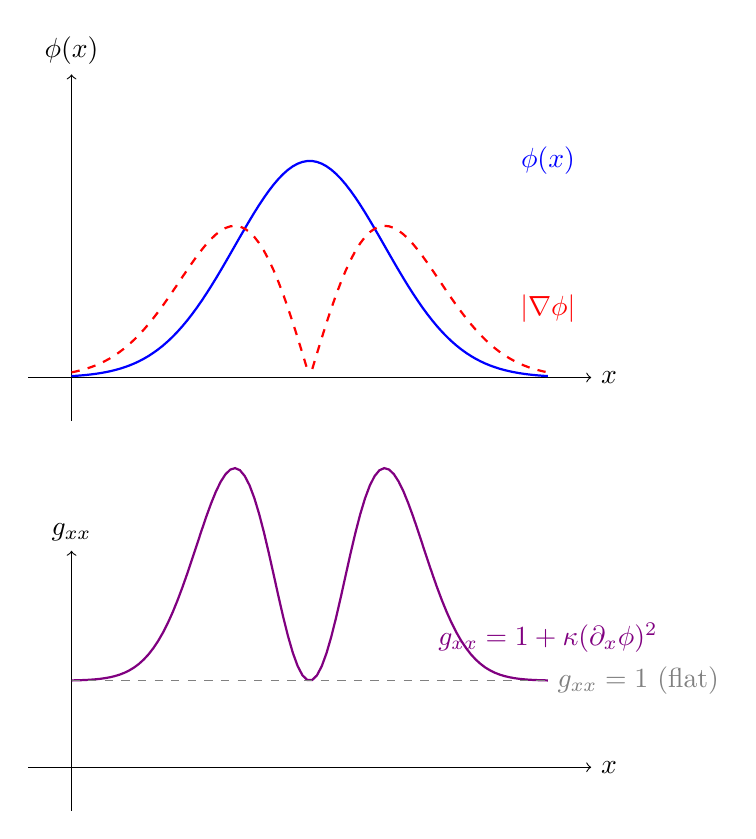
\begin{tikzpicture}[scale=1.1]
  % Field configuration
  \begin{scope}
    \draw[->] (-0.5,0) -- (6,0) node[right] {$x$};
    \draw[->] (0,-0.5) -- (0,3.5) node[above] {$\phi(x)$};

    % Scalar field profile (Gaussian)
    \draw[thick, blue, domain=0:5.5, samples=100] plot (\x, {2.5*exp(-(\x-2.75)^2/1.5)});
    \node[blue] at (5.5, 2.5) {$\phi(x)$};

    % Field gradient (derivative)
    \draw[thick, red, dashed, domain=0:5.5, samples=100] plot (\x, {abs(-2.5*(2*(\x-2.75)/1.5)*exp(-(\x-2.75)^2/1.5))});
    \node[red] at (5.5, 0.8) {$|\nabla \phi|$};
  \end{scope}

  % Induced metric visualization
  \begin{scope}[yshift=-4.5cm]
    \draw[->] (-0.5,0) -- (6,0) node[right] {$x$};
    \draw[->] (0,-0.5) -- (0,2.5) node[above] {$g_{xx}$};

    % Metric component
    \draw[thick, violet, domain=0:5.5, samples=100] plot (\x, {1 + 0.8*(-2.5*(2*(\x-2.75)/1.5)*exp(-(\x-2.75)^2/1.5))^2});
    \node[violet] at (5.5, 1.5) {$g_{xx} = 1 + \kappa (\partial_x \phi)^2$};

    % Flat reference
    \draw[thin, gray, dashed] (0,1) -- (5.5,1) node[right] {$g_{xx} = 1$ (flat)};
  \end{scope}
\end{tikzpicture}
\caption{Emergent metric from scalar field configuration. Field gradient $|\nabla \phi|$ (top, red dashed) induces metric correction $g_{xx} = 1 + \kappa (\partial_x \phi)^2$ (bottom, violet), creating effective curvature where field varies rapidly.}
\label{fig:p3:emergent_metric}
\end{figure}

\marginxref{Figure~\ref{fig:p3:emergent_metric} shows 1D example. In 3D, field "walls" or "bubbles" create localized curvature, potentially trapping matter or light.}

%------------------------------------------------------------------------------
\section{Effective Dimensions from Renormalization Group}
\label{sec:p3:effective_dimensions}
%------------------------------------------------------------------------------

\subsection{RG Flow and Scale-Dependent Dimensionality}

The renormalization group (RG) describes how physical parameters change with energy scale $\mu$. Effective spacetime dimension can also "run":
\begin{equation}
  \mu \frac{d D_{\text{eff}}}{d\mu} = \beta_D(\mu)
  \label{eq:p3:dimension_rg_flow}
\end{equation}
where $\beta_D$ is the dimensional beta function.
\marginmath{Dimensional flow: $\beta_D > 0$ indicates UV dimension increase (high energy reveals extra dimensions). $\beta_D < 0$ indicates IR reduction (low energy hides dimensions).}

\textbf{Fixed points}: Values of $D_{\text{eff}}^*$ where $\beta_D(D^*) = 0$:
\begin{itemize}
  \item IR fixed point: $D^*_{\text{IR}} = 4$ (observable 4D spacetime)
  \item UV fixed point: $D^*_{\text{UV}} = 10$ (string theory fundamental dimension)
\end{itemize}
\marginphysics{Physical meaning: at low energies, effective dimension flows to 4D. At Planck scale, full 10D (or 11D in M-theory) structure becomes accessible.}

\begin{figure}[htbp]
\centering
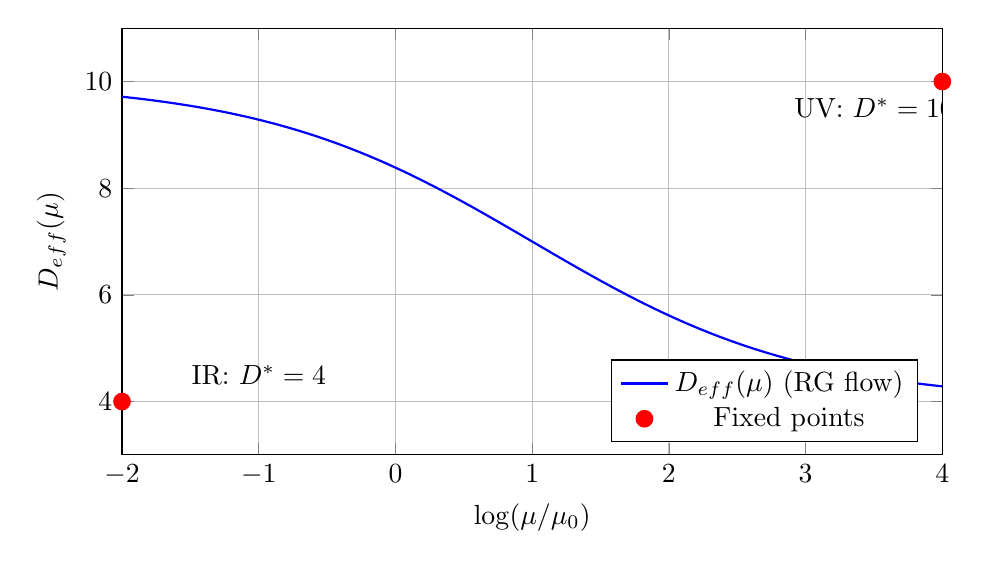
\begin{tikzpicture}
  \begin{axis}[
    width=12cm, height=7cm,
    xlabel={$\log(\mu/\mu_0)$},
    ylabel={$D_{\text{eff}}(\mu)$},
    xmin=-2, xmax=4,
    ymin=3, ymax=11,
    grid=both,
    legend pos=south east
  ]
    % RG flow from UV to IR
    \addplot[blue, thick, domain=-2:4, samples=100] {4 + 6/(1 + exp(x-1))};
    \addlegendentry{$D_{\text{eff}}(\mu)$ (RG flow)}

    % Fixed points
    \addplot[red, only marks, mark=*, mark size=3pt] coordinates {(-2, 4) (4, 10)};
    \addlegendentry{Fixed points}

    % Annotations
    \node at (axis cs:-1, 4.5) {IR: $D^* = 4$};
    \node at (axis cs:3.5, 9.5) {UV: $D^* = 10$};
  \end{axis}
\end{tikzpicture}
\caption{Renormalization group flow of effective dimension. At low energies ($\mu \to 0$), dimension flows to IR fixed point $D^* = 4$. At high energies (Planck scale), UV fixed point $D^* = 10$ represents fundamental dimensionality.}
\label{fig:p3:rg_dimension_flow}
\end{figure}

\margincaution{RG dimensional flow is model-dependent. Different theories predict different $\beta_D$ functions and fixed points.}

\subsection{Spectral Dimension and Random Walks}

The \textbf{spectral dimension}\index{spectral dimension} $d_s$ characterizes diffusion on fractal or quantum spacetimes:
\begin{equation}
  d_s = -2 \frac{d \log P(t)}{d \log t}
  \label{eq:p3:spectral_dimension}
\end{equation}
where $P(t)$ is return probability for random walk.
\marginmath{For Euclidean $d$-dimensional space: $P(t) \sim t^{-d/2}$, giving $d_s = d$. For fractals: $d_s < d_H$ (Hausdorff dimension).}

Quantum gravity simulations (causal dynamical triangulations) find:
\begin{equation}
  d_s(\mu) = \begin{cases}
    \approx 2 & \text{at Planck scale (UV)} \\
    \approx 4 & \text{at macroscopic scales (IR)}
  \end{cases}
  \label{eq:p3:spectral_dim_running}
\end{equation}
\marginphysics{Spectral dimension drop to 2D at Planck scale suggests quantum spacetime has fractal-like microstructure, transitioning to smooth 4D at large scales.}

%------------------------------------------------------------------------------
\section{Holographic Principle and Dimensional Reduction}
\label{sec:p3:holographic}
%------------------------------------------------------------------------------

\subsection{Holographic Entropy Bound}

The \textbf{holographic principle}\index{holographic principle} states that information in a volume is encoded on its bounding surface:
\begin{equation}
  S \leq \frac{A}{4 l_P^2}
  \label{eq:p3:holographic_bound}
\end{equation}
where $S$ is entropy, $A$ is surface area, $l_P = \sqrt{G\hbar/c^3} \approx 10^{-35}$ m is Planck length.
\marginmath{Entropy scales with area, not volume---dimensional reduction! 3D physics encoded on 2D boundary.}

\marginphysics{Black hole thermodynamics: Bekenstein-Hawking entropy $S_{BH} = A/(4l_P^2)$ saturates holographic bound. Black holes are maximally entropic objects.}

\subsection{AdS/CFT Correspondence}

The \textbf{Anti-de Sitter/Conformal Field Theory (AdS/CFT) correspondence}\index{AdS/CFT} provides explicit holographic realization:
\begin{equation}
  \text{Quantum gravity in AdS}_{d+1} \quad \longleftrightarrow \quad \text{CFT on boundary}^d
  \label{eq:p3:ads_cft}
\end{equation}
\marginhistory{Maldacena's 1997 AdS/CFT conjecture revolutionized theoretical physics, providing first concrete example of holography and quantum gravity/gauge theory duality.}

\textbf{Dictionary} (AdS bulk $\leftrightarrow$ CFT boundary):
\begin{itemize}
  \item Bulk metric $g_{\mu\nu}$ $\leftrightarrow$ Boundary stress-energy tensor $T_{\mu\nu}$
  \item Bulk scalar field $\phi$ $\leftrightarrow$ Boundary operator $\mathcal{O}$ with scaling dimension $\Delta$
  \item Bulk black hole $\leftrightarrow$ Thermal state in CFT
\end{itemize}
\marginmath{Scaling dimension $\Delta$ relates to bulk mass via $m^2 L^2 = \Delta(\Delta - d)$ where $L$ is AdS radius.}

\begin{figure}[htbp]
\centering
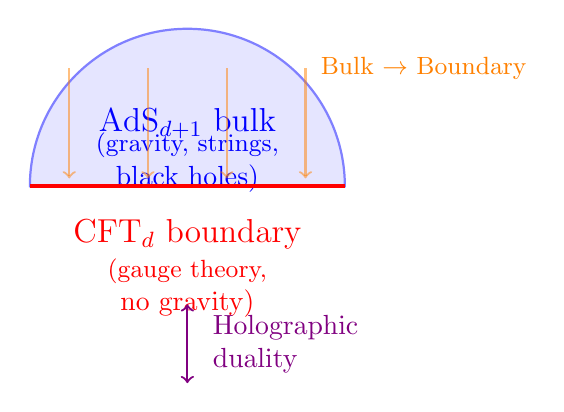
\begin{tikzpicture}[scale=1.0]
  % AdS bulk (schematic)
  \draw[thick, blue!50, fill=blue!10] (0,0) -- (4,0) arc (0:180:2) -- cycle;
  \node[blue] at (2, 0.8) {\large AdS$_{d+1}$ bulk};
  \node[blue, align=center] at (2, 0.3) {\small (gravity, strings,\\black holes)};

  % Boundary CFT
  \draw[ultra thick, red] (0,0) -- (4,0);
  \node[red, below] at (2, -0.3) {\large CFT$_d$ boundary};
  \node[red, below, align=center] at (2, -0.8) {\small (gauge theory,\\no gravity)};

  % Holographic mapping
  \draw[<->, thick, violet] (2, -1.5) -- (2, -2.5);
  \node[violet, right, align=left] at (2.2, -2) {Holographic\\duality};

  % Information flow
  \foreach \x in {0.5, 1.5, 2.5, 3.5} {
    \draw[->, thick, orange, opacity=0.5] (\x, 1.5) -- (\x, 0.1);
  }
  \node[orange] at (5, 1.5) {\small Bulk $\to$ Boundary};
\end{tikzpicture}
\caption{AdS/CFT holographic correspondence. Quantum gravity in $(d+1)$-dimensional Anti-de Sitter space (blue bulk) is dual to conformal field theory on $d$-dimensional boundary (red). Bulk physics encodes on lower-dimensional boundary.}
\label{fig:p3:ads_cft_schematic}
\end{figure}

\marginxref{Figure~\ref{fig:p3:ads_cft_schematic} illustrates holographic projection. Boundary CFT contains complete information about bulk gravity---dimensional reduction in action.}

%------------------------------------------------------------------------------
\section{Induced Geometry on Field Manifolds}
\label{sec:p3:field_manifolds}
%------------------------------------------------------------------------------

\subsection{Configuration Space Geometry}

For field $\phi: M \to \mathbb{R}$, the space of all field configurations $\mathcal{C} = \{\phi\}$ forms infinite-dimensional manifold.
\marginmath{Configuration space $\mathcal{C}$ is function space with metric induced from field theory action.}

\textbf{DeWitt metric} on configuration space:
\begin{equation}
  G_{\phi\phi'}[\delta\phi] = \int_M \sqrt{g} \, g^{\mu\nu} \delta\phi(x) \nabla_\mu \nabla_\nu \delta\phi'(x) \, d^dx
  \label{eq:p3:dewitt_metric}
\end{equation}
where $\delta\phi$ is field variation.
\marginmath{Metric on field space: measures "distance" between field configurations. Geodesics in $\mathcal{C}$ are classical field trajectories (equations of motion).}

\subsection{Moduli Space and Vacuum Manifolds}

For theories with spontaneous symmetry breaking, vacuum configurations form \textbf{moduli space}\index{moduli space} $\mathcal{M}_{\text{vac}}$:
\begin{equation}
  \mathcal{M}_{\text{vac}} = \{\phi_{\text{vac}} : V(\phi_{\text{vac}}) = V_{\min}\} / G
  \label{eq:p3:moduli_space}
\end{equation}
where $V(\phi)$ is potential and $G$ is gauge/symmetry group.
\marginphysics{Moduli space geometry determines vacuum degeneracy, domain walls, cosmic strings, and moduli stabilization in string compactifications.}

\textbf{Example: Mexican hat potential}:
\begin{equation}
  V(\phi) = \lambda (\phi^2 - v^2)^2
  \label{eq:p3:mexican_hat}
\end{equation}
Vacuum manifold: $|\phi_{\text{vac}}| = v$, a circle $S^1$ with circumference $2\pi v$.
\marginex{Higgs mechanism: $\phi$ rolls down Mexican hat potential, spontaneously breaking $U(1)$ symmetry. Vacuum choice along circle determines gauge boson masses.}

%------------------------------------------------------------------------------
\section{Dimensional Reduction via Field Condensates}
\label{sec:p3:condensates}
%------------------------------------------------------------------------------

\subsection{Dimensional Compactification from Condensates}

Consider 5D theory with scalar field $\Phi(x^\mu, y)$ where $y$ is extra dimension. If $\Phi$ develops vacuum expectation value (VEV):
\begin{equation}
  \langle \Phi(y) \rangle = \Phi_0 e^{iky}
  \label{eq:p3:condensate_vev}
\end{equation}
with $k = 1/R$, the vacuum becomes periodic with period $2\pi R$, effectively compactifying $y$ on circle.
\marginmath{Condensate-driven compactification: field VEV spontaneously selects compactification radius $R = 1/k$ via energy minimization.}

\marginphysics{Differs from Kaluza-Klein: here compactification emerges dynamically from field dynamics, not imposed by hand.}

\subsection{Topology Change via Phase Transitions}

Field configurations can induce topology change. Consider Einstein-Hilbert action with scalar:
\begin{equation}
  S = \int d^4x \sqrt{-g} \left[ \frac{R}{16\pi G} - \frac{1}{2}(\partial\phi)^2 - V(\phi) \right]
  \label{eq:p3:gravity_scalar_action}
\end{equation}

For specific potentials $V(\phi)$, solutions exist with changing topology (wormholes, bubble nucleation).
\margincaution{Topology-changing solutions typically require exotic matter (violating energy conditions) or quantum tunneling. Classical topology change is highly constrained.}

%------------------------------------------------------------------------------
\section{Emergent Symmetries and Conservation Laws}
\label{sec:p3:emergent_symmetries}
%------------------------------------------------------------------------------

\subsection{Noether's Theorem and Emergent Currents}

Symmetries need not be fundamental---they can emerge at low energies. For action $S[\phi]$ approximately invariant under $\phi \to \phi + \delta\phi$:
\begin{equation}
  \delta S = \int d^dx \, \mathcal{L}_{\text{breaking}} \ll S
  \label{eq:p3:approximate_symmetry}
\end{equation}

\textbf{Approximate Noether current}:
\begin{equation}
  j^\mu = \frac{\partial \mathcal{L}}{\partial(\partial_\mu \phi)} \delta\phi - \mathcal{J}^\mu_{\text{breaking}}
  \label{eq:p3:approximate_current}
\end{equation}
with $\partial_\mu \mathcal{J}^\mu_{\text{breaking}} = \mathcal{L}_{\text{breaking}}$.
\marginmath{Emergent symmetry: at energies $E \ll E_{\text{break}}$, symmetry breaking term $\mathcal{L}_{\text{breaking}}$ negligible. Symmetry appears exact, with conserved current $\partial_\mu j^\mu \approx 0$.}

\textbf{Example: Chiral symmetry in QCD}:
At energies $E \gg m_{\text{quark}}$, quark masses negligible. QCD Lagrangian has approximate $SU(2)_L \times SU(2)_R$ chiral symmetry, spontaneously broken to $SU(2)_V$ (isospin), giving rise to pions as pseudo-Goldstone bosons.
\marginphysics{Emergent chiral symmetry explains pion properties (low mass, pseudoscalar) despite QCD having no exact chiral symmetry at fundamental level.}

%------------------------------------------------------------------------------
\section{Quantum-to-Classical Transition}
\label{sec:p3:quantum_classical}
%------------------------------------------------------------------------------

\subsection{Decoherence and Geometric Emergence}

Smooth classical geometry emerges from quantum superpositions via decoherence\index{decoherence}:
\begin{equation}
  |\psi\rangle = \sum_i c_i |g_i\rangle \quad \xrightarrow{\text{decoherence}} \quad \rho = \sum_i |c_i|^2 |g_i\rangle\langle g_i|
  \label{eq:p3:decoherence}
\end{equation}
where $|g_i\rangle$ are different geometric (metric) states.
\marginmath{Decoherence: environment-induced loss of quantum coherence converts superposition (pure state $|\psi\rangle$) to classical mixture (density matrix $\rho$).}

\textbf{Emergent classicality condition}:
Decoherence timescale $\tau_{\text{dec}}$ must be much shorter than observation time $\tau_{\text{obs}}$:
\begin{equation}
  \tau_{\text{dec}} \ll \tau_{\text{obs}}
  \label{eq:p3:classicality_condition}
\end{equation}
\marginphysics{For macroscopic objects, $\tau_{\text{dec}} \sim 10^{-40}$ s (essentially instantaneous). Quantum superpositions of different geometries decohere immediately, yielding definite classical spacetime.}

\begin{figure}[htbp]
\centering
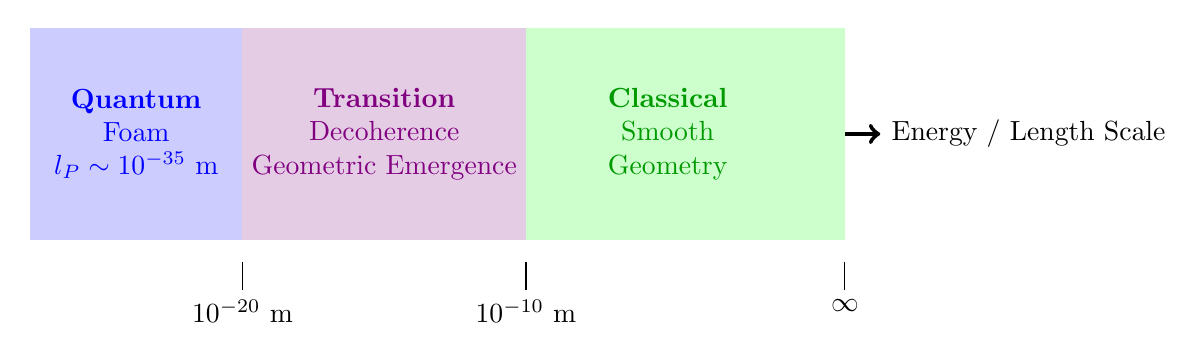
\begin{tikzpicture}[scale=0.9]
  % Energy scale axis
  \draw[->, ultra thick] (0,0) -- (12,0) node[right] {Energy / Length Scale};

  % Quantum regime
  \fill[blue!20] (0,-1.5) rectangle (3,1.5);
  \node[blue, align=center] at (1.5, 0) {\textbf{Quantum}\\Foam\\$l_P \sim 10^{-35}$ m};

  % Transition regime
  \fill[violet!20] (3,-1.5) rectangle (7,1.5);
  \node[violet, align=center] at (5, 0) {\textbf{Transition}\\Decoherence\\Geometric Emergence};

  % Classical regime
  \fill[green!20] (7,-1.5) rectangle (11.5,1.5);
  \node[green!60!black, align=center] at (9, 0) {\textbf{Classical}\\Smooth\\Geometry};

  % Scale markers
  \draw (3, -1.8) -- (3, -2.2) node[below] {$10^{-20}$ m};
  \draw (7, -1.8) -- (7, -2.2) node[below] {$10^{-10}$ m};
  \draw (11.5, -1.8) -- (11.5, -2.2) node[below] {$\infty$};
\end{tikzpicture}
\caption{Quantum-to-classical transition for spacetime geometry. At Planck scale (blue), quantum fluctuations dominate. Through decoherence (violet), superpositions collapse. At macroscopic scales (green), smooth classical geometry emerges.}
\label{fig:p3:quantum_classical_transition}
\end{figure}

\marginxref{Figure~\ref{fig:p3:quantum_classical_transition} depicts energy/scale regimes. Emergent geometry is classical limit of underlying quantum theory.}

%------------------------------------------------------------------------------
\section{Summary and Forward Bridge}
\label{sec:p3:ch3_summary}
%------------------------------------------------------------------------------

This chapter explored how geometric structures emerge from underlying field dynamics:

\textbf{Key Mechanisms}:
\begin{itemize}
  \item \textbf{Induced metrics} (Eq.~\ref{eq:p3:induced_metric}): Field gradients generate effective spacetime curvature
  \item \textbf{RG dimensional flow} (Eq.~\ref{eq:p3:dimension_rg_flow}): Effective dimension runs with energy scale
  \item \textbf{Holographic principle} (Eq.~\ref{eq:p3:holographic_bound}): 3D information encoded on 2D surface
  \item \textbf{AdS/CFT} (Eq.~\ref{eq:p3:ads_cft}): Explicit gravity/gauge duality exhibiting holography
  \item \textbf{Decoherence} (Eq.~\ref{eq:p3:decoherence}): Quantum-to-classical transition yielding definite geometry
\end{itemize}

\textbf{Physical Insights}:
\begin{itemize}
  \item Geometry is not fundamental but emergent from field configurations
  \item Spacetime dimension varies with energy scale (spectral dimension)
  \item Bulk physics encodes on lower-dimensional boundaries (holography)
  \item Classical smoothness emerges via decoherence of quantum fluctuations
\end{itemize}

\marginxref{Chapter~\ref{ch:p3:field_dynamics} applies these ideas to field dynamics and scaling laws, investigating critical phenomena and universality.}

Wheeler's vision of geometry emerging from quantum dynamics finds concrete realization in holography, RG flow, and decoherence mechanisms. Chapter~\ref{ch:p3:field_dynamics} extends this to field dynamics on fractal structures, exploring how scaling laws and critical phenomena govern behavior at multiple scales.

%==============================================================================
% END OF CHAPTER 3
%==============================================================================
